% ----------------------------------
% Cap Análisis
% ----------------------------------
%	Incluye
%		Casos de uso
%
\documentclass[a4paper,oneside,11pt]{book}

\usepackage[spanish,activeacute]{babel}
\usepackage[utf8]{inputenc}
%\usepackage[T1]{fontenc}
\usepackage{tabulary}
\usepackage{graphicx}
\usepackage{color}
\usepackage{colortbl}
\usepackage{float}

\oddsidemargin=0.2cm
\headsep=1cm
\textheight=21cm
\textwidth=16cm

\setcounter{secnumdepth}{3}

\definecolor{gris}{gray}{0.80}
\definecolor{gris2}{gray}{0.90}
\definecolor{negro}{gray}{0}

% Personalizamos la separación entre párrafos...
\parskip=6pt

% Personalizamos el identado en la primera línea del nuevo párrafo...
\parindent=10pt

\begin{document}
	
\chapter{Diseño} % (fold)
\label{cha:diseno}

	
	\section{Diagrama de clases} % (fold)
	\label{sec:diagrama_de_clases}
	
		Un \textbf{diagrama de clases} es un tipo de diagrama estático que describe la estructura de un sistema mostrando sus clases, atributos y las relaciones entre ellos. Los diagramas de clases son utilizados durante el proceso de análisis y diseño de los sistemas, donde se crea el diseño conceptual de la información que se manejará en el sistema, y los componentes que se encargaran del funcionamiento y la relación entre uno y otro.
		
		Existen una serie de conceptos que tenemos que tener bastante claros. En primer lugar las \textbf{propiedades también llamados atributos o características}, son valores que corresponden a un objeto, como color, material, cantidad, ubicación. Generalmente se conoce como la información detallada del objeto. Suponiendo que el objeto es una puerta, sus propiedades serían: la marca, tamaño, color y peso.	El siguiente concepto son las \textbf{operaciones comúnmente llamados métodos}, son aquellas actividades o verbos que se pueden realizar con/para este objeto, como por ejemplo abrir, cerrar, buscar, cancelar, acreditar, cargar. De la misma manera que el nombre de un atributo, el nombre de una operación se escribe con minúsculas si consta de una sola palabra. Si el nombre contiene más de una palabra, cada palabra será unida a la anterior y comenzará con una letra mayúscula, a excepción de la primera palabra que comenzará en minúscula. Por ejemplo: abrirPuerta, cerrarPuerta, buscarPuerta, etc. Otro concepto es el de \textbf{interfaz}, que es un conjunto de operaciones que permiten a un objeto comportarse de cierta manera, por lo que define los requerimientos mínimos del objeto. Hace referencia a polimorfismo. Y por último el concepto de \textbf{herencia}, que se define como la reutilización de un objeto padre ya definido para poder extender la funcionalidad en un objeto hijo. Los objetos hijos heredan todas las operaciones y/o propiedades de un objeto padre. Anotar que los atributos y los métodos pueden ser privados, públicos o protegidos, permitiendo así ser accedidos o no por objetos de su misma o de otras clases. 
		
		Debemos tener conocimiento, además, de que a la hora de diseñar se suelen utilizar \textbf{patrones de diseño}, los cuales brindan una solución ya probada y documentada a problemas de desarrollo de software que están sujetos a contextos similares. Debemos tener presente los siguientes elementos de un patrón: su nombre, el problema (cuando aplicar un patrón), la solución (descripción abstracta del problema) y las consecuencias (costos y beneficios).
		
		El proyecto que nos atañe se basa en el \textit{framework rails}, que corre en el lenguaje de programación \textit{ruby}. \textit{Ruby on Rails} se basa en el patrón de diseño\textbf{Modelo Vista Controlador (MVC)}, que es un patrón de arquitectura de software que separa los datos de una aplicación, la interfaz de usuario, y la lógica de control en tres componentes distintos. El patrón de llamada y retorno MVC (según CMU), se ve frecuentemente en aplicaciones web como la que nos ocupa, donde \textbf{la vista} es la página HTML y el código que provee de datos dinámicos a la página. \textbf{El modelo} es el Sistema de Gestión de Base de Datos y la Lógica de negocio, y \textbf{el controlador} es el responsable de recibir los eventos de entrada desde la vista. 	
		
		Muchos de los sistemas informáticos utilizan un Sistema de Gestión de Base de Datos para gestionar los datos: en líneas generales del MVC corresponde al modelo. La unión entre capa de presentación y capa de negocio conocido en el paradigma de la Programación por capas representaría la integración entre Vista y su correspondiente Controlador de eventos y acceso a datos, MVC no pretende discriminar entre capa de negocio y capa de presentación pero si pretende separar la capa visual gráfica de su correspondiente programación y acceso a datos, algo que mejora el desarrollo y mantenimiento de la Vista y el Controlador en paralelo, ya que ambos cumplen ciclos de vida muy distintos entre sí.
		
		Aunque se pueden encontrar diferentes implementaciones de MVC, el flujo que sigue \textit{rails} es el siguiente:
		
		\begin{figure}[H]
		  \centering
		    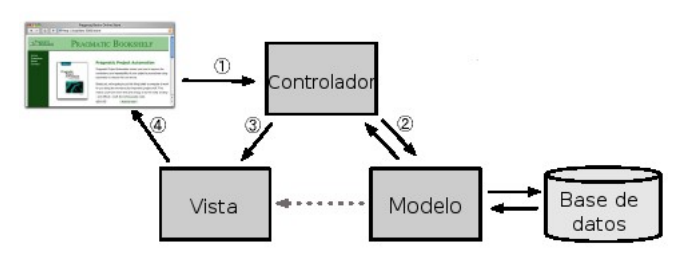
\includegraphics[width=16cm]{img/png/mvc.png}
		  \caption{Flujo Patrón Modelo Vista Controlador}
		  \label{fig:patron_mvc}
		\end{figure}
		
		\begin{enumerate}
			\item El usuario interactúa con la interfaz de usuario de alguna forma (por ejemplo, el usuario pulsa un botón, enlace, etc.). Entonces, el navegador envía una petición.
			\item El controlador recibe (por parte de los objetos de la interfaz-vista) la notificación de la acción solicitada por el usuario. El controlador gestiona el evento que llega. Entonces, el controlador accede al modelo (interactúa con el modelo), actualizándolo, posiblemente modificándolo de forma adecuada a la acción solicitada por el usuario (por ejemplo, el controlador actualiza los datos de un médico). Los controladores complejos están a menudo estructurados usando un patrón de comando que encapsula las acciones y simplifica su extensión.
			\item Los controladores invocan a las vistas.
			\item La vista \textit{dibuja} la siguiente página para el navegador.
			\item La interfaz de usuario espera nuevas interacciones del usuario, comenzando el ciclo nuevamente.
		\end{enumerate}
		
		A continuación el diagrama de clases (Figura \ref{fig:dis_clases}).
		
		\begin{figure}[H]
		  \centering
		    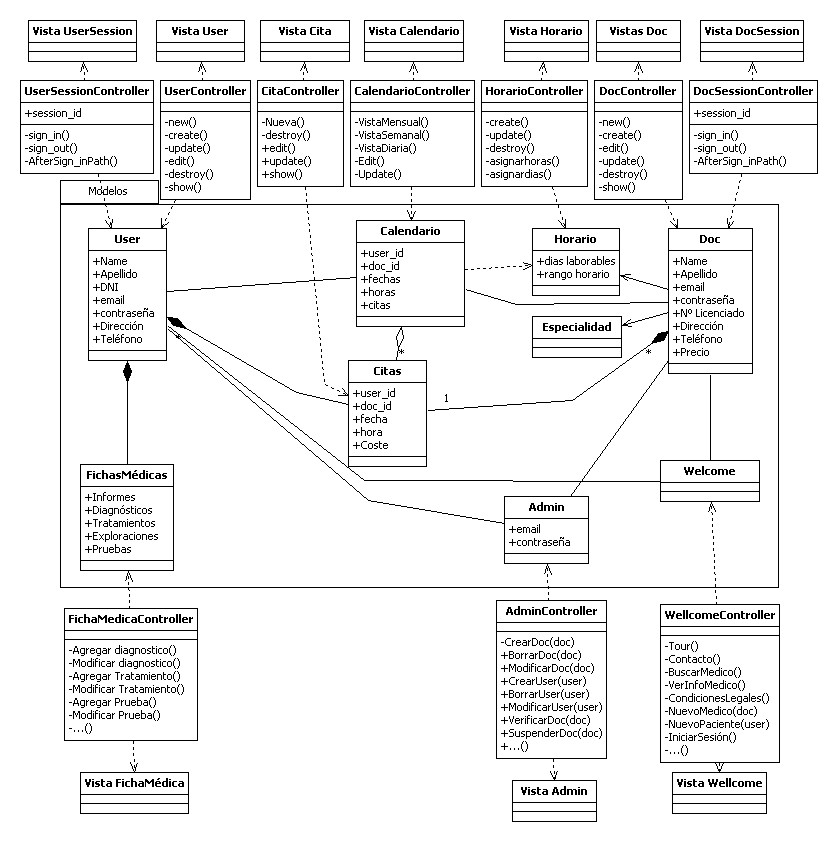
\includegraphics[width=16cm]{img/jpg/dis_clases/clases.jpg}
		  \caption{Diagrama de clases}
		  \label{fig:dis_clases}
		\end{figure}
		
	% section diagrama_de_clases (end)
	
	\newpage
	\section{Diagramas de secuencia} % (fold)
\label{sec:diagramas_de_secuencia}

	Cómo fue explicado en capítulos anteriores, los diagramas de interacción son diagramas que describen cómo grupos de objetos colaboran para conseguir algún fin. Estos diagramas muestran objetos, así como los mensajes que se pasan entre ellos dentro del caso de uso, es decir, capturan el comportamiento de los casos de uso.
	
	Hay dos tipos de diagrama de interacción, ambos basados en la misma información, pero cada uno enfatizando un aspecto particular: \textbf{Diagramas de Secuencia} y Diagramas de Colaboración.

	\medskip
	
	\fcolorbox{negro}{gris}{\parbox{15cm}{Un \textit{diagrama de Secuencia} muestra una interacción ordenada según la secuencia temporal de eventos. En particular, muestra los objetos participantes en la interacción y los mensajes que intercambian ordenados según su secuencia en el tiempo. Es decir, muestra la interacción de un conjunto de objetos en una aplicación a través del tiempo y se modela para cada caso de uso.}}
	
	\medskip
	
	En cuanto a la \textbf{representación}, el eje vertical representa el tiempo, y en el eje horizontal se colocan los objetos y actores participantes en la interacción, sin un orden prefijado. Cada objeto o actor tiene una línea vertical, y los mensajes se representan mediante flechas entre los distintos objetos. El tiempo fluye de arriba abajo. Se pueden colocar etiquetas (como restricciones de tiempo, descripciones de acciones, etc.) bien en el margen izquierdo o bien junto a las transiciones o activaciones a las que se refieren. 
	
	En este documento se detallan dos diagramas de secuencia hacen referencia a las \textit{Actividades Generales}. Son el de \textit{Buscar médico} y \textit{Ver información del médico.} Recordar que se utiliza el patrón de diseño modelo-vista-controlador.

	\newpage
	\subsection{Actividades generales} % (fold)
	\label{sub:actividades_generales}
	
		En primer lugar el diagrama de secuencia relacionado con el caso de uso \textit{Buscar médico}. En el interfaz principal de la aplicación, cuyo archivo para las vistas es \textit{index.html.erb}, nos aparece un cuadro de búsqueda en el que introducir los datos que deseamos, en este caso, el nombre y los apellidos del médico. La búsqueda se envía al controlador de dicha interfaz principal (\textit{welcome controller}), concretamente a la función \textit{search result}, y éste realiza una petición en la tabla \textit{doc}.
		
		Para realizar dicha petición, se unen previamente las columnas de \textit{name + apellido} de la tabla \textit{doc}, y luego se realiza la búsqueda. Por último, es este mismo controlador  (\textit{welcome controller}) el que se encarga de actualizar la vista del \textit{index.html.erb} mostrando los resultados obtenidos.
		
		\bigskip
		\bigskip
		
		\begin{figure}[H]
		  \centering
		    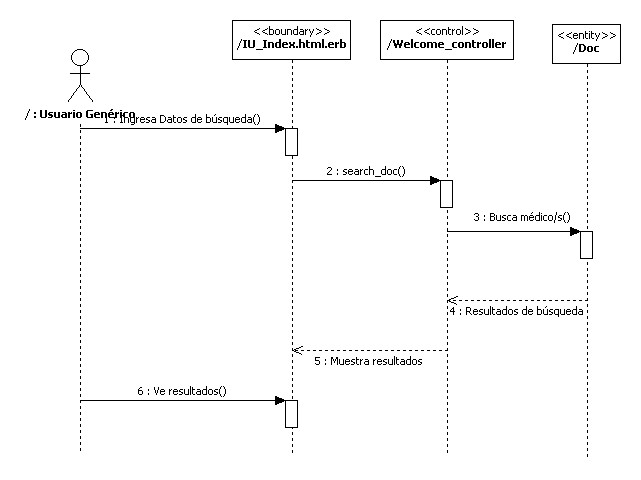
\includegraphics[width=16cm]{img/jpg/secuencia/01_BuscarMedico.jpg}
		  \caption{Buscar médico}
		  \label{fig:sec_general_buscarmedico}
		\end{figure}
		\newpage
		El segundo caso de uso llevado a estudio, y que posteriormente será implementado, es el de poder ver la información referente a un médico. Para ello, en la interfaz principal debemos previamente realizar una búsqueda. Los resultados obtenidos (médicos encontrados en función del nombre y apellidos introducidos) son \textit{links} en los que podemos hacer \textit{click} para acceder a ver la información.
		
		En este caso, el interfaz notificará al controlador \textit{doc controller} que el usuario ha seleccionado ver la información de un médico. Para ello se utiliza la acción \textit{show} del controlador. Se buscará el médico en la tabla \textit{doc} y a continuación se mostrará la vista relacionada con dicha acción, es decir, el \textit{show.html.erb} del médico seleccionado.
		\begin{figure}[H]
		  \centering
		    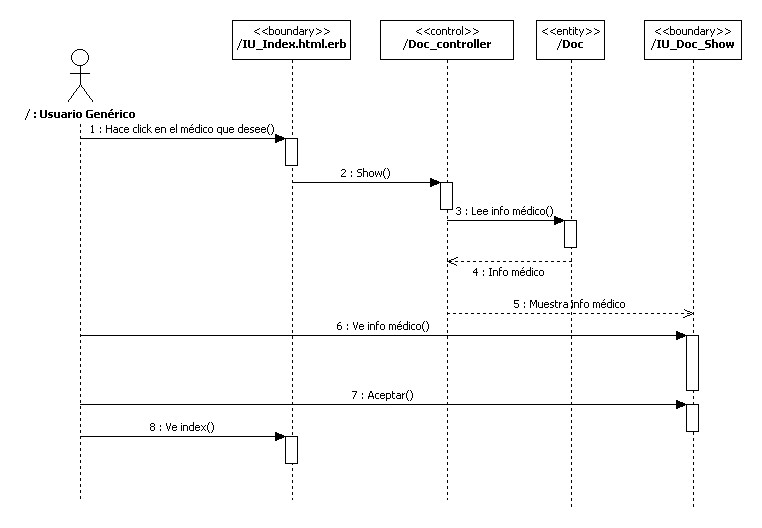
\includegraphics[width=16cm]{img/jpg/secuencia/02_VerInfoMedico.jpg}
		  \caption{Ver información del médico}
		  \label{fig:sec_general_verinfomedico}
		\end{figure}
		
	% subsection actividades_generales (end)
	
% section diagramas_de_secuencia (end)
		
	\newpage
	\section{Diagrama de capas} % (fold)
	\label{sec:diagrama_de_capas}
	
		Como ya vimos en análisis, cualquier sistema grande se debe dividir en unidades más pequeñas, de modo que las personas puedan trabajar con una cantidad de información limitada, a la vez y de modo que los equipos de trabajo no interfieran con el trabajo de los otros. La gestión del modelo consiste en paquetes y relaciones de dependencia de los paquetes.
		
		Un paquete es, por tanto, una parte de un modelo. Además, cada parte de un modelo debe pertenecer a un paquete. El modelador puede asignar el contenido de un modelo a un conjunto de paquetes. Pero, para ser funcional, la asignación debe seguir un cierto principio racional, tal como funcionalidad común, implementación estrechamente relacionada, y un punto de vista común.
		
		En nuestro caso, vamos a agrupar los paquetes en base a tres capas. \textbf{La capa específica, la capa genérica y la capa Middleware. (Figura \ref{fig:dcapas}}. No es necesario que utilicemos la capa del sistema.
		
		En la primera, se hace mención a los paquetes propios de la aplicación, como son todos aquellos relacionados con las \textit{Actividades de los médicos, de los pacientes, de las fichas médicas, del administrador y de los usuarios genéricos.} Además, todos estos paquetes se dividen en subpaquetes, para agrupar una serie de actividades más específicas de cada uno de ellos. 
		
		Por su parte, en la segunda, se agrupan una serie de paquetes que pueden ser reutilizados en otras aplicaciones. En este proyecto son los relacionados con el \textit{registro de usuarios, algunas librerías javascript, la función autocompletar, la posibilidad de realizar paginación y todo lo relacionado con el multilenguaje.}
		
		En la tercera, vemos en más detalle las gemas utilizadas que dan sustento a las capas superiores.
		
		Una vez visto el diagrama general dividido en tres capas principales, con los subsistemas(paquetes) que contienen cada una de ellas, vamos a ver con más detalle los paquetes de la capa específica.
		
		En primer lugar, el paquete de \textit{Actividades de los médicos} (Figura \ref{fig:dcapas_medicos}), que está compuesto por \textit{Gestión del horario, del calendario, de los pacientes, de las plantillas, de las estadísticas y la administración.}
		
		A continuación tenemos los paquetes en los que están divididas las \textit{Actividades de los pacientes} (Figura \ref{fig:dcapas_pacientes}), que son \textit{la Gestión del calendario, de los médicos y de las fichas médicas.}
		
		Por último, vemos los paquetes que forman las \textit{Fichas médicas} (Figura \ref{fig:dcapas_fichas}). Éstos son \textit{Gestión de antecedentes, de informes, de tratamientos, de exploraciones, de pruebas y de observaciones}.
		
		\begin{figure}[H]
		  \centering
		    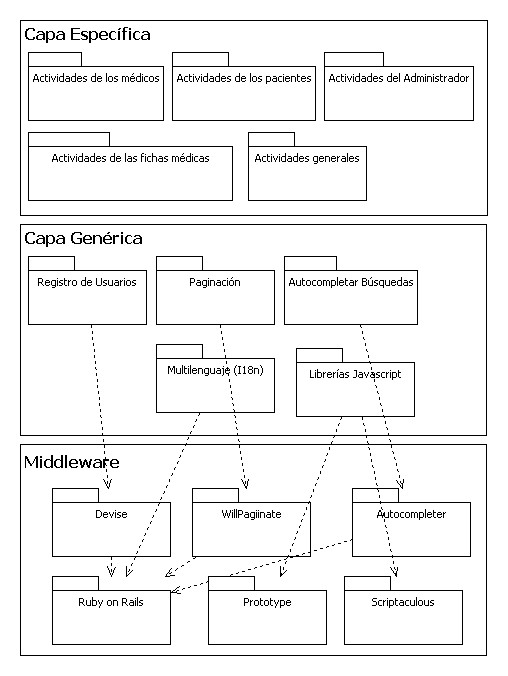
\includegraphics[width=16cm]{img/jpg/dcapas/capas.jpg}
		  \caption{Diagrama de Capas}
		  \label{fig:dcapas}
		\end{figure}
		
		
		
		\begin{figure}[H]
		  \centering
		    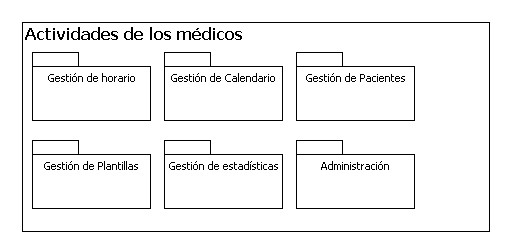
\includegraphics[width=12cm]{img/jpg/dcapas/Actividades_medicos.jpg}
		  \caption{Diagrama de Capas}
		  \label{fig:dcapas_medicos}
		\end{figure}
		
		\begin{figure}[H]
		  \centering
		    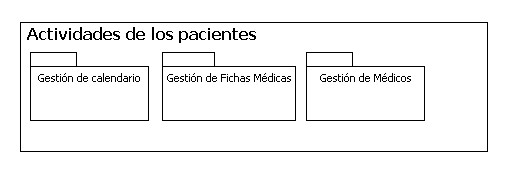
\includegraphics[width=12cm]{img/jpg/dcapas/Actividades_Pacientes.jpg}
		  \caption{Diagrama de Capas}
		  \label{fig:dcapas_pacientes}
		\end{figure}
		
		\begin{figure}[H]
		  \centering
		    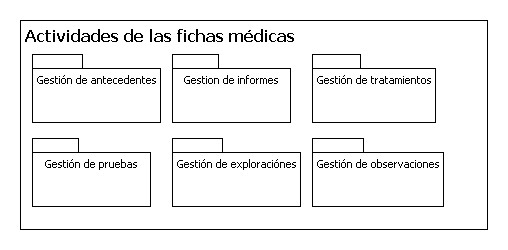
\includegraphics[width=12cm]{img/jpg/dcapas/fichas_medicas.jpg}
		  \caption{Diagrama de Capas}
		  \label{fig:dcapas_fichas}
		\end{figure}

		
	
	% section diagrama_de_capas (end)
	
	\newpage
	\section{Diagrama de despliegue} % (fold)
	\label{sec:diagrama_de_despliegue}
	
		Un diagrama de despliegue muestra la configuración de los nodos de proceso y las instancias de componentes y objetos que residen en ellos. Los componentes representan unidades de código de ejecución. Los componentes que no existen como entidades de ejecución (porque se han compilado aparte) no aparecen en estos diagramas; deben aparecer en diagramas de componentes.
		
		\fcolorbox{negro}{gris}{\parbox{15cm}{Un Diagrama de Despliegue modela la arquitectura en tiempo de ejecución de un sistema. Esto muestra la configuración de los elementos de hardware (nodos) y muestra cómo los elementos y artefactos del software se trazan en esos nodos. Es decir se sitúa el software en el hardware que lo contiene. Cada Hardware se representa como un nodo.}}
		
		Los elementos usados por este tipo de diagrama son nodos (representados como un prisma), componentes (representados como una caja rectangular con dos protuberancias del lado izquierdo) y asociaciones.
	
		A continuación (Figura \ref{fig:despliegue}) podemos ver el diagrama de despliegue, que destaca por tener en un lado el equipo del cliente, y en el otro, el servidor de aplicación y de bases de datos.
		
			\begin{figure}[H]
			  \centering
			    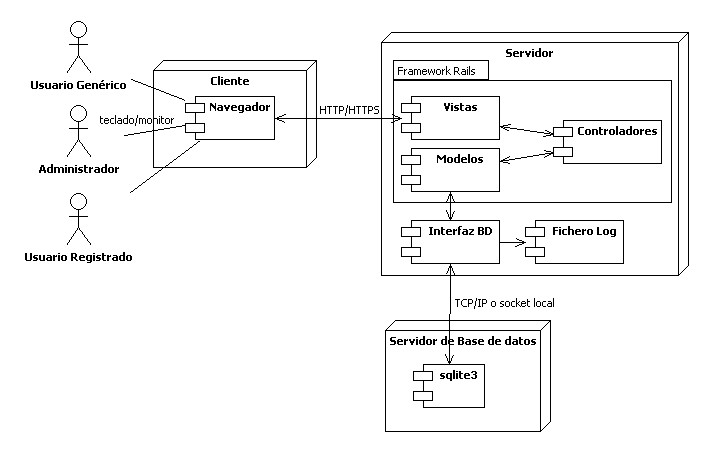
\includegraphics[width=16cm]{img/jpg/despliegue/despliegue.jpg}
			  \caption{Diagrama de Despliegue}
			  \label{fig:despliegue}
			\end{figure}
		
	
	% section diagrama_de_despliegue (end)
% chapter análisis (end)

\end{document}